\documentclass[runningheads]{llncs}
\usepackage[T1]{fontenc}
\usepackage[utf8]{inputenc}
\usepackage{lmodern}
\usepackage{graphicx,booktabs,longtable,array,calc,amsmath,amssymb}
\usepackage[hidelinks]{hyperref}
\providecommand{\tightlist}{\setlength{\itemsep}{0pt}\setlength{\parskip}{0pt}}
\def\LTcaptype{table}
\makeatletter\setlength{\LTcapwidth}{\textwidth}
\def\LT@makecaption#1#2#3{\LT@mcol\LT@cols c{\hbox to\z@{\hss\parbox[t]\LTcapwidth{\small\textbf{#2.} #3\par\vskip0.4\baselineskip}\hss}}}
\makeatother
\setlength{\emergencystretch}{1em}
\renewcommand{\thetable}{S\arabic{table}}
\renewcommand{\thefigure}{S\arabic{figure}}
\begin{document}
\title{Supplementary Material. GPU-accelerated single-cell (NVIDIA DGX H100) and spatial (RTX 4090) transcriptomics: per-step speedups, capacity and concordance against a 100-CPU reference}
\titlerunning{Supplementary Material}
\author{Luca Vedovelli\inst{1,2} \and Corrado Lanera\inst{1,2} \and Daniele Sabbatini\inst{1,2,3} \and Dario Gregori\inst{1,2}}
\authorrunning{L. Vedovelli et al.}
\institute{Unit of Biostatistics, Epidemiology and Public Health, Department of Cardiac, Thoracic, Vascular Sciences and Public Health, University of Padova, Padova, Italy. \\ \email{\{luca.vedovelli,\allowbreak{}corrado.lanera,\allowbreak{}daniele.sabbatini,\allowbreak{}dario.gregori\}@ubep.unipd.it} \and
BIOSTAT-X, Biostatistics \& AI for Biomedical Discovery, Pediatric Research Institute ``Città della Speranza'', Padova, Italy \and
Neuromuscular Unit, Department of Neuroscience, University of Padova, Padova, Italy}
\maketitle

\hypertarget{overview}{%
\section{Overview}\label{overview}}

This document accompanies the chapter. It contains the extended methods with Supplementary Tables S1-S3, the extended results with Supplementary Tables S4-S8 and Supplementary Figures S1-S3, and an extended discussion of the points not covered in the chapter. References of the form ``Table 1 of the chapter'' point to the chapter; section names in quotation marks refer to the sections of this document.

\hypertarget{supplementary-methods}{%
\section{Supplementary Methods}\label{supplementary-methods}}

\hypertarget{dataset-and-subsampling}{%
\subsection{Dataset and subsampling}\label{dataset-and-subsampling}}

All single-cell experiments used mouse brain cells from the CZ CELLxGENE Census (release 2025-11-08) \cite{CZCellxGene2025}: primary-data cells (\texttt{is\_\allowbreak{}primary\_\allowbreak{}data}) with \texttt{tissue\_\allowbreak{}general} = brain profiled with 10x Genomics 3' chemistry (v1 to v3), 3,436,470 cells in total. For the scaling benchmark we drew 1,300,000 of these cells uniformly at random without replacement (seed = 42).

To evaluate performance across scales, we created reproducible subsamples of 50,000, 100,000 and 500,000 cells from the 1.3M-cell sample by uniform random sampling without replacement (\texttt{numpy.random.choice}, seed = 42); the 10,000-cell set was drawn in the same way (seed = 42) directly from the Census selection in a preliminary test job, and the 1.3M-cell sample itself was the largest size.
All subsamples were therefore drawn from the same Census selection, so that the expected biological composition is the same across benchmarking tiers.

\hypertarget{analysis-pipeline}{%
\subsection{Analysis pipeline}\label{analysis-pipeline}}

Both the CPU and GPU pipelines implemented the standard Scanpy workflow (cf. \cite{Luecken2019,Heumos2023}) with the same parameter values, except for the implementation-specific settings listed in Table S1 (Leiden iterations, PCA solver and neighbour search).
The CPU pipeline used Scanpy 1.12 \cite{Wolf2018} with NumPy 2.2.6 and the igraph Leiden backend (igraph 1.0.0); the GPU pipeline used rapids-singlecell 0.14.1 \cite{Dicks2026} with CuPy 13.6.0, the RAPIDS Memory Manager (RMM) 26.2.0, and the cuGraph Leiden backend.
Both pipelines shared the AnnData format \cite{Virshup2024} for data interchange.

The pipeline comprised ten steps (Table S1), timed with \texttt{time.perf\_\allowbreak{}counter()}; in the CPU and single-GPU pipelines scaling (step 5) was timed together with PCA (step 6), whereas the multi-GPU configuration timed scaling and the host-to-GPU transfer as separate steps, and each of the three Leiden resolutions had its own timer. The reported total is the sum of the timed steps, not the wall-clock time of the job: RMM initialisation, the GPU warm-up, the copy of \texttt{adata.raw}, HVG subsetting and Dask cluster start-up and shutdown were not timed.

{\footnotesize\setlength{\tabcolsep}{2pt}
\begin{longtable}[]{@{}
  >{\raggedleft\arraybackslash}p{(\columnwidth - 6\tabcolsep) * \real{0.1111}}
  >{\raggedright\arraybackslash}p{(\columnwidth - 6\tabcolsep) * \real{0.2037}}
  >{\raggedright\arraybackslash}p{(\columnwidth - 6\tabcolsep) * \real{0.2963}}
  >{\raggedright\arraybackslash}p{(\columnwidth - 6\tabcolsep) * \real{0.3889}}@{}}
\caption{\label{tab:S1}Pipeline steps, parameters, and implementations for the scRNA-seq benchmark. All steps used identical parameters for the CPU and GPU pipelines except where noted.}\tabularnewline
\toprule\noalign{}
\begin{minipage}[b]{\linewidth}\raggedleft
Step
\end{minipage} & \begin{minipage}[b]{\linewidth}\raggedright
Operation
\end{minipage} & \begin{minipage}[b]{\linewidth}\raggedright
Key parameters
\end{minipage} & \begin{minipage}[b]{\linewidth}\raggedright
Implementation note
\end{minipage} \\
\midrule\noalign{}
\endfirsthead
\toprule\noalign{}
\begin{minipage}[b]{\linewidth}\raggedleft
Step
\end{minipage} & \begin{minipage}[b]{\linewidth}\raggedright
Operation
\end{minipage} & \begin{minipage}[b]{\linewidth}\raggedright
Key parameters
\end{minipage} & \begin{minipage}[b]{\linewidth}\raggedright
Implementation note
\end{minipage} \\
\midrule\noalign{}
\endhead
\bottomrule\noalign{}
\endlastfoot
1 & Data loading & n.a. & \texttt{read\_\allowbreak{}h5ad()} from disk \\
2 & QC and filtering & \texttt{min\_\allowbreak{}genes} = 200, \texttt{min\_\allowbreak{}cells} = 3, mt prefix = \texttt{mt-} & Mitochondrial percentage calculated, cells/genes filtered \\
3 & Normalisation & \texttt{target\_\allowbreak{}sum} = 10,000 & Library-size scaling + \texttt{log1p} \\
4 & HVG selection & \texttt{n\_\allowbreak{}top\_\allowbreak{}genes} = 2,000, Seurat v1 method & On log-normalised data \cite{Satija2015,Yip2019} \\
5 & Scaling & \texttt{max\_\allowbreak{}value} = 10 & Sparse to dense float32, mean-centre, unit-variance; timed with PCA in the CPU and single-GPU pipelines \\
6 & PCA & 50 components, seed = 42 & CPU: scikit-learn PCA (ARPACK) on the dense scaled matrix; GPU: cuML PCA (default solver) \\
7 & Neighbour graph & k = 15, 50 PCs, seed = 42 & k-NN in PCA space; CPU: pynndescent (Scanpy default from 8,192 cells, \texttt{n\_\allowbreak{}jobs} = 1); GPU: brute-force k-NN (rapids-singlecell default) \\
8 & Leiden clustering & r in \{0.5, 1.0, 1.5\}, seed = 42; \texttt{n\_\allowbreak{}iterations} = 2 (CPU) / 100 (GPU, rapids-singlecell default) & igraph (CPU) / cuGraph (GPU) \cite{Traag2019} \\
9 & UMAP & 2 components, seed = 42 & 2D embedding \cite{McInnes2018} \\
10 & DE testing & Wilcoxon, one-vs-rest, \texttt{use\_\allowbreak{}raw} = True & On Leiden r = 1.0 clusters \cite{Soneson2018} \\
\end{longtable}
}

For the CPU pipeline, \texttt{OMP\_\allowbreak{}NUM\_\allowbreak{}THREADS}, \texttt{MKL\_\allowbreak{}NUM\_\allowbreak{}THREADS}, \texttt{OPENBLAS\_\allowbreak{}NUM\_\allowbreak{}THREADS} and \texttt{NUMBA\_\allowbreak{}NUM\_\allowbreak{}THREADS} were set to 100, the number of CPUs (hardware threads) allocated by SLURM, before any numerical library was imported, so that the OpenMP, BLAS and Numba thread pools used by NumPy, SciPy, scikit-learn and umap-learn were all sized to the allocation. Neighbour search was the exception: from 8,192 cells upward, that is at every benchmark size, Scanpy 1.12 builds the k-NN graph with pynndescent and passes it the Scanpy default \texttt{n\_\allowbreak{}jobs} = 1, so Numba ran on one thread during this step. In a separate measurement on the spatial GPU workstation (PCA embeddings recomputed from the 10,000-, 50,000- and 100,000-cell benchmark files; five repeats per setting, one process each, timing the call after JIT compilation), \texttt{n\_\allowbreak{}jobs} = 100 made this step 1.16, 1.91 and 2.48 times faster than \texttt{n\_\allowbreak{}jobs} = 1.
For single-GPU runs, RMM was initialised at the start of each repeat with a pool allocator (initial pool 50\% and maximum 100\% of device memory, the RMM defaults), which also served the CuPy allocations: the out-of-memory error of the single-GPU pipeline at 500,000 cells was raised by this pool. Before timing, a 100 $\times$ 100 matrix product created the CUDA context; it does not compile the rapids-singlecell kernels, so the first repeat also includes JIT compilation. The wall-clock interval between consecutive repeats, an upper bound on the untimed overhead because it also includes writing the results, was 8.2 s against 2.5 s of timed steps for one GPU at 10,000 cells (means of repeats 2-5: the first repeat has no preceding timestamp, so this figure is the one exception to the five-repeat convention).

\hypertarget{multi-gpu-configuration}{%
\subsection{Multi-GPU configuration}\label{multi-gpu-configuration}}

At every dataset size we also ran a hybrid configuration with a Dask \cite{Rocklin2015} and Dask-CUDA \cite{RAPIDS2024} cluster of 2, 4 or 8 workers, one per GPU, each with a 10 GB initial / 70 GB maximum RMM pool. Data loading, QC, normalisation and HVG selection ran in Scanpy on the host CPU, and the HVG-subset matrix was then transferred to GPU 0 as a CuPy array. Because it was not converted to a Dask array, scaling, PCA, neighbour search, Leiden, UMAP and DE all ran on GPU 0, and the additional GPUs did not take part in the computation; rapids-singlecell 0.14.1 provides Dask-based routes for QC metrics, total-count normalisation, scaling and PCA, among other steps, which this configuration did not use. The 8-GPU runs ran on a different node from the 1-, 2- and 4-GPU runs (Section ``Hardware and software environment''). Results at 500k and 1.3M cells come only from this configuration, because the single-GPU pipeline failed during QC at these sizes (at 500k cells an allocation of 23.8 GiB exceeded the RMM pool, whose maximum is the whole device memory; at 1.3M cells QC stopped with a CUDA illegal-memory-access error).

\hypertarget{concordance-metrics}{%
\subsection{Concordance metrics}\label{concordance-metrics}}

To assess whether the GPU pipeline produces biologically equivalent results, we selected six concordance metrics covering five stages of the analysis pipeline (two for clustering), such that a divergence at any stage would be detected independently of the others (Table S2). The panel progresses from upstream operations (feature selection, dimensionality reduction) through graph and clustering steps to downstream differential expression. ARI is used as a clustering metric in published scRNA-seq benchmarks \cite{Tian2019,Duo2020,Luecken2022}, NMI and an HVG overlap score in \cite{Luecken2022} and a kNN Jaccard in \cite{Gardner2025}; the PCA and DE metrics were defined for this study.

{\footnotesize\setlength{\tabcolsep}{2pt}
\begin{longtable}[]{@{}
  >{\raggedright\arraybackslash}p{(\columnwidth - 4\tabcolsep) * \real{0.2963}}
  >{\raggedright\arraybackslash}p{(\columnwidth - 4\tabcolsep) * \real{0.4444}}
  >{\raggedright\arraybackslash}p{(\columnwidth - 4\tabcolsep) * \real{0.2593}}@{}}
\caption{\label{tab:S2}Concordance metrics used to compare CPU and GPU pipeline outputs. Concordance was computed once, at 10,000 cells, on a separate pair of CPU and GPU runs made on 11 March 2026 (UTC) in a preliminary test job (16 CPUs, one GPU), with the same input file and parameters as the benchmark but before the timed repeats; at Leiden r = 1.0 and 1.5 its CPU run found 40 and 45 clusters, against 41 and 46 in all five timed CPU repeats.}\tabularnewline
\toprule\noalign{}
\begin{minipage}[b]{\linewidth}\raggedright
Metric
\end{minipage} & \begin{minipage}[b]{\linewidth}\raggedright
Definition
\end{minipage} & \begin{minipage}[b]{\linewidth}\raggedright
Scope
\end{minipage} \\
\midrule\noalign{}
\endfirsthead
\toprule\noalign{}
\begin{minipage}[b]{\linewidth}\raggedright
Metric
\end{minipage} & \begin{minipage}[b]{\linewidth}\raggedright
Definition
\end{minipage} & \begin{minipage}[b]{\linewidth}\raggedright
Scope
\end{minipage} \\
\midrule\noalign{}
\endhead
\bottomrule\noalign{}
\endlastfoot
HVG Jaccard & size of intersection divided by size of union of the CPU and GPU gene sets for 2,000 HVGs & Feature selection \\
PCA loading $|\rho|$ & Mean absolute Spearman $\rho$ across first 10 PC loadings, accounting for sign flips & Dimensionality reduction \\
kNN Jaccard & Mean per-cell Jaccard overlap of the CPU and GPU neighbour index sets (k = 15) as stored by each pipeline (CPU sets: 16 indices, GPU sets: 15, both including the cell itself); a stability metric also used in \cite{Gardner2025} & Graph structure \\
ARI & Adjusted Rand Index of Leiden cluster assignments, adjusted for chance \cite{Hubert1985} & Clustering \\
NMI & Normalised Mutual Information of cluster assignments \cite{Vinh2010} & Clustering \\
DE logFC $\rho$ & Spearman $\rho$ of log-fold-changes of the top 100 CPU DE genes of each cluster against the GPU values for the same genes, averaged over CPU-GPU cluster pairs matched with the Hungarian algorithm on shared cells (Leiden r = 1.0); metric defined for this study & Differential expression \\
\end{longtable}
}

\hypertarget{stress-test-maximum-capacity}{%
\subsection{Stress test: maximum capacity}\label{stress-test-maximum-capacity}}

To determine the maximum dataset size processable on a single DGX H100 node, we implemented a memory-optimised pipeline variant. The stress test used the 3,436,470-cell Census selection described above (and random subsets of it at 1.7M and 3.4M cells, seed = 42). Larger sizes were built by concatenating whole copies of the dataset, with renamed cell identifiers, plus a random draw of the remaining cells (6.9M cells: 2 copies; 10.3M: 3 copies; 11.9M: 3 copies plus 1,590,590 cells), so duplicated cells are present in the expression matrix and in the k-NN graph. Because duplicated cells reach the \texttt{min\_\allowbreak{}cells} = 3 threshold, the number of genes passing QC grew with replication (41,344 at 3.44M, 42,394 at 6.87M and 44,158 from 10.3M cells). At 3,436,470, 6,872,940 and 10,309,410 cells, cuML KMeans with k = 50, 100 and 200 replaced the three Leiden resolutions. DE was skipped (\texttt{-\/-skip-de}) at every size except 1.7M and 3.4M cells.
The key optimisations were: (i) scaling on CPU rather than GPU (leveraging 2 TB system RAM); (ii) a covariance PCA in which the parent process scattered the scaled matrix across the 8 GPUs, computed per-GPU partial products (2,000 $\times$ 2,000), summed and eigendecomposed them on GPU 0 and projected locally; the matrix was not re-centred after clipping at \texttt{max\_\allowbreak{}value} = 10 and partial products were accumulated in float32, so the result approximates, but is not identical to, standard PCA; (iii) lean GPU transfer that replaces the dense matrix with an empty sparse placeholder after PCA, since downstream steps (neighbours, clustering, UMAP) only require the PCA embedding; and (iv) a reduced RMM pool (2 GB) for each Dask-CUDA worker; the workers were started but performed no computation.
We ran the memory-optimised pipeline at 15 sizes from 3.4M to 11.9M cells, refining the step size towards the failure point; single attempts at 12.0M and 13.7M cells (4 copies of the dataset) did not complete. Two further variants were run: a sparse-scatter variant computes per-gene mean and standard deviation from the sparse matrix on CPU and lets each GPU densify and scale its own chunk, so the dense matrix never exists on CPU; a chunked variant selects HVGs from per-gene statistics accumulated over 100,000-cell batches and computes PCA by batch-wise covariance accumulation. CPU memory was recorded as the resident set size of the parent Python process (\texttt{psutil.Process().memory\_\allowbreak{}info().rss}), sampled immediately before and after each pipeline step, with an explicit garbage collection before each pre-step sample; the reported peak is the maximum over these post-step samples. This instrumentation yields a lower bound on the job's true memory use for two reasons: it cannot observe allocations that are made and released within a single step, and it excludes the resident memory of the eight Dask-CUDA worker processes, which the SLURM cgroup does account for. The replication of the dataset for sizes above 3,436,470 cells ran between data loading and QC, outside any timed step: at 11.9M cells it accounts for the 302.34 GiB increase between these two samples, and its transient peak was not sampled. GPU memory was recorded with NVML as device memory in use, summed over the eight GPUs; it includes the RMM pools of the Dask-CUDA workers. All memory values are in GiB (bytes / 1024\^{}3).

\hypertarget{differential-expression-at-scale}{%
\subsection{Differential expression at scale}\label{differential-expression-at-scale}}

DE was benchmarked on a 3,400,000-cell random subset of the Census selection (seed = 42; 3,399,892 cells and 41,321 genes in \texttt{adata.raw} after QC). Differential expression testing at atlas scale is constrained by hardware, which shaped the design of this benchmark. The matrix used for DE, \texttt{adata.raw.X}, holds log-normalised values rather than raw counts in this pipeline, and the GPU tests processed it in gene chunks, either scattered across GPUs or streamed through a single GPU. We timed six DE configurations (Table S6): a t-test on CPU (Scanpy); a t-test and a Wilcoxon test with gene chunks scattered across 8 GPUs; the same two tests with gene chunks streamed through one GPU; and pseudo-bulk aggregation followed by a Wilcoxon test on CPU. A Wilcoxon test on CPU was not run at this size and pseudo-bulk was not run on GPU, so the design is not a full factorial. In the scatter strategy a single host thread processed the chunks in sequence, alternating devices, so the GPUs did not work concurrently. Gene chunks of 500 were used for GPU strategies, giving 500 $\times$ 3.4M $\times$ 4 bytes approximately 6.8 GB per chunk, well within the 80 GB per-device limit. The GPU tests were custom CuPy kernels, not \texttt{rank\_\allowbreak{}genes\_\allowbreak{}groups}: the Wilcoxon kernel assigned ordinal ranks without averaging ties and computed neither p-values nor a multiple-testing correction, so it yields a rank-sum statistic used here for timing only. GPU timings start after \texttt{adata.raw.X} was converted to CSC format, whereas CPU timings cover the whole \texttt{rank\_\allowbreak{}genes\_\allowbreak{}groups} call. Pseudo-bulk aggregation summed the values of \texttt{adata.raw.X} over donor $\times$ cluster groups (Census \texttt{donor\_\allowbreak{}id}, 202 donors; groups with fewer than 5 cells discarded; 2,431 pseudo-samples over 81 clusters), re-normalised the sums to counts per million, applied a second log transformation and compared clusters with a Wilcoxon test. We use this aggregation as a timing proxy for pseudo-bulk analysis; count-based methods such as edgeR or DESeq2 are recommended for pseudo-bulk DE between conditions \cite{Squair2021}.

\hypertarget{spatial-datasets}{%
\subsection{Spatial datasets}\label{spatial-datasets}}

Spatial benchmarks used two 10x Genomics public datasets, both obtained from the 10x Genomics public data portal. The first is Visium v1 Mouse Brain Sagittal Anterior, the standard spot-based spatial transcriptomics platform, consisting of 2,695 spots at 55~\textmu{}m resolution and approximately 32,285 genes. The second is the Visium HD Spatial Gene Expression Library, Mouse Brain (FFPE), processed by 10x Genomics with Space Ranger 3.0.0 (CytAssist; Visium Mouse Transcriptome Probe Set v2.0), benchmarked at two bin sizes: 8~\textmu{}m (393,543 bins) and 2~\textmu{}m (6,296,688 bins, randomly subsampled to 400,000 bins with seed 42; 389,492 after QC), each quantifying 19,059 genes. The Visium HD 2~\textmu{}m dataset was subsampled to 400,000 bins using the \texttt{-\/-max-spots} flag so that the benchmark would fit within the RTX 4090's 24 GB VRAM. Random subsampling kept 6.35\% of the 2~\textmu{}m bins, so the subsample has the bin density of a regular grid with a spacing of about 8~\textmu{}m, and its spatial neighbour graph and autocorrelation statistics do not describe the native 2~\textmu{}m resolution.

\hypertarget{spatial-analysis-pipeline}{%
\subsection{Spatial analysis pipeline}\label{spatial-analysis-pipeline}}

The spatial pipeline comprised two phases: an expression analysis phase (shared with the scRNA-seq pipeline) and a spatial statistics phase (Table S3).

{\footnotesize\setlength{\tabcolsep}{2pt}
\begin{longtable}[]{@{}
  >{\raggedleft\arraybackslash}p{(\columnwidth - 6\tabcolsep) * \real{0.1622}}
  >{\raggedright\arraybackslash}p{(\columnwidth - 6\tabcolsep) * \real{0.2973}}
  >{\centering\arraybackslash}p{(\columnwidth - 6\tabcolsep) * \real{0.3514}}
  >{\raggedright\arraybackslash}p{(\columnwidth - 6\tabcolsep) * \real{0.1892}}@{}}
\caption{\label{tab:S3}Spatial analysis pipeline steps. Steps 1-8 share parameters with the scRNA-seq pipeline (Table S1) except for QC filtering, which used \texttt{min\_\allowbreak{}genes} = 1 for Visium HD (Space Ranger pre-filters on-tissue barcodes). Steps 9-14 are spatial-specific.}\tabularnewline
\toprule\noalign{}
\begin{minipage}[b]{\linewidth}\raggedleft
Step
\end{minipage} & \begin{minipage}[b]{\linewidth}\raggedright
Operation
\end{minipage} & \begin{minipage}[b]{\linewidth}\centering
GPU support
\end{minipage} & \begin{minipage}[b]{\linewidth}\raggedright
Notes
\end{minipage} \\
\midrule\noalign{}
\endfirsthead
\toprule\noalign{}
\begin{minipage}[b]{\linewidth}\raggedleft
Step
\end{minipage} & \begin{minipage}[b]{\linewidth}\raggedright
Operation
\end{minipage} & \begin{minipage}[b]{\linewidth}\centering
GPU support
\end{minipage} & \begin{minipage}[b]{\linewidth}\raggedright
Notes
\end{minipage} \\
\midrule\noalign{}
\endhead
\bottomrule\noalign{}
\endlastfoot
1-8 & Expression analysis (QC through UMAP) & Yes & As in Table S1; Leiden r = 1.0 for Visium, r = 0.1 for HD \\
9 & Spatial neighbours & No & Delaunay triangulation (scipy.spatial) \\
10 & Moran's I & Yes & Spatial autocorrelation per gene \\
11 & Geary's C & Yes & Spatial autocorrelation per gene \\
12 & Co-occurrence & Yes & Cluster co-occurrence across distance intervals \\
13 & Neighbourhood enrichment & No & Cluster-cluster proximity enrichment \\
14 & Ligand-receptor interaction & Not used & Squidpy re-implementation of CellPhoneDB \cite{Palla2022}; the GPU version in rapids-singlecell 0.14.1 was not used \\
\end{longtable}
}

The CPU baseline used Scanpy 1.12 for expression steps and Squidpy 1.8.1 \cite{Palla2022} for spatial steps.
The GPU pipeline used rapids-singlecell 0.14.1 for both expression and GPU-accelerated spatial steps (Moran's I, Geary's C, co-occurrence).
Spatial neighbours and neighbourhood enrichment, which have no GPU implementation in rapids-singlecell 0.14.1, and ligand-receptor analysis, whose GPU implementation in rapids-singlecell 0.14.1 (\texttt{rsc.gr.ligrec}) our GPU pipeline did not use, ran in Squidpy on the CPU in both pipelines. On Visium HD (more than 8,192 bins), CPU expression neighbour search used pynndescent with one Numba thread, as in the scRNA-seq CPU pipeline.

Co-occurrence and neighbourhood enrichment were skipped when the number of cell groups exceeded 500, because their memory grows with the square of the number of groups, and ligand-receptor analysis was skipped above 100,000 spots. These limits, and the Leiden resolution of 0.1 used above 100,000 spots (that is, for Visium HD), were practical choices to keep memory and run time tractable; we did not test their sensitivity.

\hypertarget{spatial-concordance-metrics}{%
\subsection{Spatial concordance metrics}\label{spatial-concordance-metrics}}

We compared CPU and GPU spatial outputs along five axes. Spatial autocorrelation concordance was measured as the Spearman $\rho$ between CPU and GPU per-gene Moran's I (and separately Geary's C) statistics across the 2,000 highly variable genes on which spatial autocorrelation was computed. Spatially variable gene (SVG) Jaccard overlap was computed for the top-N SVGs ranked by Moran's I (with N taking the values 50, 100, and 200) and for the complete set of genes passing FDR \textless{} 0.05. Clustering agreement was assessed by the adjusted Rand index and normalised mutual information of Leiden cluster assignments from the expression-based pipeline. Co-occurrence and neighbourhood enrichment concordance were the Spearman $\rho$ between the full CPU and GPU matrices, computed on the same cell groups; for co-occurrence we also counted the distance intervals at which the CPU and GPU matrices agreed within an absolute tolerance of 0.001. Each metric was computed for the five pairs of CPU repeat k and GPU repeat k; we report the value when it is the same in all pairs and the range otherwise. To check the GPU co-occurrence at Visium HD 8~\textmu{}m, we repeated it alone five times on the same cell groups, with rapids-singlecell 0.15.1 and, as a control, 0.14.1, in images that differ only in this package.

\hypertarget{hardware-and-software-environment}{%
\subsection{Hardware and software environment}\label{hardware-and-software-environment}}

Single-cell benchmarks ran on DGX H100 nodes of the UPSCALE/CONVECS cluster at the University of Padova; each node has 8 $\times$ NVIDIA H100 80 GB SXM GPUs connected via NVLink 4.0, two Intel Xeon Platinum 8480C CPUs (112 cores, 224 hardware threads) and 2 TB of DDR5 RAM.
The software environment was encapsulated in a Singularity container built from the NVIDIA RAPIDS base image (\nolinkurl{nvcr.io/nvidia/rapidsai/base:26.02-cuda12-py3.12}).
Key software versions: Scanpy 1.12, rapids-singlecell 0.14.1, CuPy 13.6.0, Dask 2026.1.1, Dask-CUDA 26.2.0, Python 3.12.12.
Jobs were submitted via SLURM without exclusive allocation. The single-GPU, 2-GPU and 4-GPU benchmarks ran concurrently on node \texttt{poddgx01} (NVIDIA driver 535.247.01) with 16, 32 and 56 allocated CPUs, and the 8-GPU benchmark ran at the same time on node \texttt{poddgx02} (driver 535.183.01) with 100 CPUs, as many as the CPU baseline, which ran earlier on \texttt{poddgx01}. The stress test and the DE benchmark were pinned to \texttt{poddgx02} with 200 CPUs (100 for the 1.7M-cell stress-test run).

GPU spatial benchmarks ran on a workstation with an NVIDIA GeForce RTX 4090 (24 GB) and an AMD Ryzen Threadripper PRO 5995WX CPU (64 cores, 128 threads). The CPU reference ran on DGX node \texttt{poddgx02}, reserved exclusively, as a SLURM step with 100 CPUs (50 physical cores with two hardware threads each), the same number of CPUs as the scRNA-seq CPU baseline; the workstation CPU at 128 threads was measured as a control. CPU reference and GPU therefore ran on different machines. The NVIDIA driver of the workstation was 580.126.09 for preliminary runs in March 2026 and 595.99.02 for the runs reported here; GPU times of the steps that do not depend on the cell groups changed by a factor of 0.94 to 1.04 between the two.
The spatial container was built on the same \nolinkurl{nvcr.io/nvidia/rapidsai/base:26.02-cuda12-py3.12} image as the scRNA-seq container, with Squidpy 1.8.1 \cite{Palla2022} and spatialdata \cite{Marconato2024} added on top for the spatial pipeline.
The GPU part of the spatial pipeline was run only on the workstation: on DGX node \texttt{poddgx02} (driver 535.183.01) a container based on RAPIDS 24.06 passed basic CuPy, RMM and rapids-singlecell tests, but smoke tests of the spatial GPU pipeline in it failed when CuPy initialised cuSPARSE and cuRAND, and the cause was not investigated further.

Each benchmark configuration was run five times; we report the mean~$\pm$~sample standard deviation (n = 5, ddof = 1) of all five repeats, and speedups are ratios of means. The five scRNA-seq repeats ran in the same process, so the first includes JIT compilation and library loading (for example, CPU neighbour search at 10k cells took 19.90 s in the first repeat and 1.12 s on average in the others). Peak RAM and VRAM are means of per-repeat peaks. The stress test, the DE benchmark and the concordance analysis were run once.
For the spatial benchmarks each repeat ran in a new process with empty Numba and CuPy JIT caches, so every repeat includes JIT compilation and, for ligand-receptor analysis, the download of the OmniPath database. Co-occurrence, neighbourhood enrichment and ligand-receptor analysis used the same cell groups in all runs, the Leiden labels of the first CPU reference repeat. Squidpy 1.8.1 sets the Numba thread count to one during neighbourhood enrichment and keeps it for the rest of the process, so ligand-receptor analysis, which follows it, ran with one Numba thread in both pipelines.

\hypertarget{reproducibility}{%
\subsection{Reproducibility}\label{reproducibility}}

All code, Dockerfiles, SLURM submission scripts and result JSON files are available at \url{https://github.com/lucavd/scRNA-DGX-benchmark} (release v1.0.0) and archived on Zenodo (\url{https://doi.org/10.5281/zenodo.23984290}). Per-cell outputs (cluster labels, HVG lists, DE tables, k-NN indices, PCA loadings, Moran's I and Geary's C values) and SLURM logs are not in the repository because of their size; the stress-test results at 1.7M and 3.4M cells and the chunked 12M-cell run were produced by intermediate versions of the scripts that were not committed.
The scRNA-seq benchmarks ran in a Singularity container built from the Docker image \nolinkurl{lucavd/sc-benchmark:latest}, whose digest was not recorded; the spatial benchmarks ran in Docker (workstation) and Apptainer (DGX CPU reference) containers from \nolinkurl{lucavd/sc-benchmark-spatial:latest} (image id sha256:738c8cc7301590c9\allowbreak{}5a3ddc3b7dd74baf\allowbreak{}eefee1f1ce188063\allowbreak{}e14a166a707a6ddd). Both images derive from \nolinkurl{nvcr.io/nvidia/rapidsai/base:26.02-cuda12-py3.12}; their Dockerfiles do not pin package versions, so the versions used are those recorded at runtime in each result file (Scanpy 1.12, rapids-singlecell 0.14.1, CuPy 13.6.0, RMM 26.2.0, NumPy 2.2.6, igraph 1.0.0).
Random seeds were fixed at 42 for all stochastic operations: subsampling (\texttt{numpy.random.choice}), PCA (\texttt{sc.pp.pca} / \texttt{rsc.pp.pca}), Leiden (\texttt{sc.tl.leiden} / \texttt{rsc.tl.leiden}), and UMAP (\texttt{sc.tl.umap} / \texttt{rsc.tl.umap}).
GPU reductions that use atomic operations can make results vary between runs because floating-point addition is not associative \cite{Collange2015,Shanmugavelu2024}. In our runs GPU Leiden labels were identical across the five repeats at 10,000 cells in every GPU configuration, but differed between repeats in every configuration from 100,000 cells upward (and in three of the four at 50,000 cells), whereas CPU labels were identical across repeats at every size. CPU-GPU differences also arise from different algorithms and settings (Leiden implementation and iterations, PCA solver, neighbour search), which the concordance metrics capture together with numerical effects.

\hypertarget{supplementary-results}{%
\section{Supplementary Results}\label{supplementary-results}}

\hypertarget{end-to-end-speedup}{%
\subsection{End-to-end speedup}\label{end-to-end-speedup}}

Table 1 of the chapter summarises the benchmark results across all 23 pipeline-dataset-GPU configurations, each averaged over five repeats.
At 1.3 million cells, the GPU pipeline with eight GPUs allocated completed the full analysis in 435.2~$\pm$~16.2 s (7.3 min), compared with 52,056.2~$\pm$~392.0 s (14.5 h) for the CPU pipeline, a 119.6-fold speedup. With two GPUs allocated the time was 493.3~$\pm$~10.3 s (105.5-fold); the difference lies in data loading (149.0 against 90.6 s, runs on different nodes), because the additional GPUs did not take part in the computation. Wilcoxon differential expression accounted for 93.5\% of the CPU time (48,688.3 s of 52,056.2 s); without it the speedup was 7.9-fold with two GPUs and 9.2-fold with eight. Dicks et al.~report, on the 10x Genomics mouse brain dataset and with differential expression and I/O excluded, more than 120-fold on one B200 GPU and 110-fold on one H200 GPU against a 32-core workstation CPU \cite{Dicks2026}; in our hybrid pipeline a similar end-to-end factor arises mainly from the CPU Wilcoxon test.
Even at 10,000 cells, the single-GPU pipeline was 12-fold faster than the CPU baseline (3.3~$\pm$~1.7 s vs 39.5~$\pm$~10.2 s).
With a single GPU the speedup grew from 12.0$\times$ at 10k to 33.7$\times$ at 50k and 43.8$\times$ at 100k. At 500k and 1.3M cells only the hybrid pipeline could run (Section ``Multi-GPU configuration''), and the speedup was 34.9$\times$ at 500k (2 GPUs) and 119.6$\times$ at 1.3M (8 GPUs; 105.5$\times$ with 2 GPUs); because the series mixes two pipelines, it is not a monotonic function of dataset size.

\hypertarget{per-step-speedup}{%
\subsection{Per-step speedup}\label{per-step-speedup}}

\begin{figure}
\centering
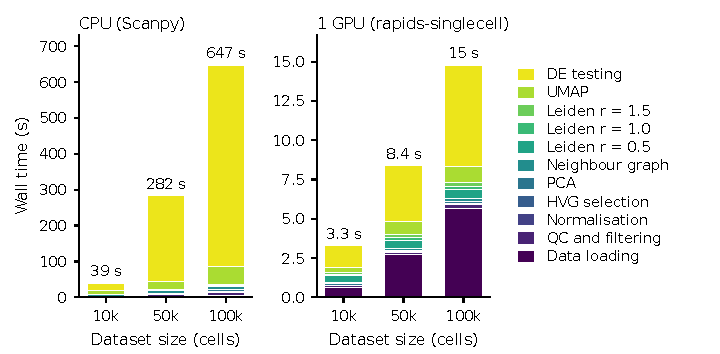
\includegraphics{figures/figS1.pdf}
\caption{\label{fig:S1}Step-level wall time decomposition for CPU vs single-GPU at 10k, 50k, and 100k cells, mean of five repeats (first repeat included); the CPU and GPU panels have separate time axes. On CPU, DE testing and UMAP dominate; on GPU, the longest step, DE testing at 100k cells, takes 6.4 s on average. CPU neighbour search ran on one Numba thread, the Scanpy default (see Methods).}
\end{figure}

Data loading was slightly slower on GPU at all three sizes (0.76-0.85$\times$, CPU time divided by GPU time). The GPU timer covers reading the file and copying the matrix to the device (\texttt{anndata\_\allowbreak{}to\_\allowbreak{}GPU}), whereas CUDA context creation and RMM pool allocation happen before the timer starts; the GPU excess grew with dataset size (0.10 s at 10k, 0.55 s at 50k and 1.38 s at 100k cells), so it is a size-dependent transfer cost rather than a fixed overhead. We note that our pipeline relies on \texttt{h5py}-based readers that route data through CPU RAM, precluding GPU Direct Storage (GDS) optimisations that would bypass the CPU entirely; this remains an avenue for future improvement. For Leiden clustering at resolution 0.5, the CPU was faster at 10k cells (0.36$\times$), but this reflects the first Leiden call of the first repeat (1.70 s against 0.09 to 0.23 s in later repeats); at resolutions 1.0 and 1.5 the GPU was already faster at 10k cells (1.36$\times$ and 1.60$\times$). At resolution 0.5 the GPU was 1.80$\times$ faster at 50k and 3.58$\times$ faster at 100k cells. The first repeat of each configuration includes one-off library loading and compilation on both CPU and GPU, and it sets the extreme per-step values at 10k cells: excluding it, normalisation was 115.1$\times$ faster on GPU (instead of 329$\times$) and Leiden at resolution 0.5 was 1.12$\times$ faster (instead of 0.36$\times$). End-to-end speedups changed by at most 6\% from 100k cells upwards.

\hypertarget{multi-gpu-configuration-1}{%
\subsection{Multi-GPU configuration}\label{multi-gpu-configuration-1}}

At 500k and 1.3M cells only the hybrid Dask-CUDA pipeline could run. In the configuration used, the expression matrix was passed to PCA and neighbour search as a CuPy array on one device, so these steps ran on a single GPU whatever the number of GPUs allocated: PCA plus neighbour search took 17.23, 16.99 and 17.01 s with 2, 4 and 8 GPUs at 1.3M cells, and 2.98, 2.97 and 3.00 s at 500k cells, where total wall time was 124.5, 125.0 and 124.6 s. At 1.3M cells the 8-GPU run (435.2 s) was 12\% faster than the 2-GPU run (493.3 s), but the difference arose in CPU-side data loading (149.0 s against 90.6 s), the jobs ran concurrently, and the 8-GPU job ran on a different node. The aggregate VRAM of the multi-GPU runs reflects the RMM pools pre-allocated by the Dask workers (78.6 GiB added at cluster start-up with 8 GPUs, at 10k as at 1.3M cells), not distributed data. Multi-GPU scaling was therefore not measured. Between 10k and 100k cells the 2-GPU hybrid pipeline was 49-82\% slower than the single-GPU pipeline, because it runs preprocessing on the CPU.

\hypertarget{concordance-at-10000-cells}{%
\subsection{Concordance at 10,000 cells}\label{concordance-at-10000-cells}}

Concordance analysis on the 10,000-cell dataset (Fig. 2 of the chapter) demonstrated that the two pipelines yield closely agreeing outputs, despite computing on different processors and hardware. Concordance was computed on a separate pair of 10,000-cell runs made on 11 March 2026 (UTC), before the timed benchmark; in that run the CPU pipeline found 31, 40 and 45 clusters at resolutions 0.5, 1.0 and 1.5, against 31, 41 and 46 in all five benchmark repeats. Upstream analysis steps showed deterministic agreement: HVG selection was perfectly concordant with all 2,000 genes identical between CPU and GPU (Jaccard = 1.000), and PCA loadings were perfectly correlated with mean absolute Spearman $\rho$ = 1.000 across all 10 inspected principal components. Neighbourhood graph construction achieved high overlap with mean Jaccard = 0.930 (median = 0.938). This value is bounded by construction: the CPU and GPU neighbour sets compared have different sizes (the maximum and the median per-cell Jaccard are both 0.9375 = 15/16, and no cell reaches 1), so at least half of the cells reach that maximum and differ only by the size mismatch. In the saved neighbour lists of the benchmark runs at 10,000 cells, identical in all five repeats, each cell has 16 CPU and 15 GPU neighbour indices, the cell itself included, and for 95.0\% of cells every GPU neighbour is also a CPU neighbour. The remaining differences are consistent with approximate neighbour search on CPU (PyNNDescent, the Scanpy default at this size) against exact brute-force search on GPU \cite{Gardner2025}, rather than with floating-point precision.

\hypertarget{memory-at-benchmark-scale}{%
\subsection{Memory at benchmark scale}\label{memory-at-benchmark-scale}}

At the scales covered by the main benchmark (10k to 1.3M cells), neither memory tier was saturated. CPU RAM grew roughly in proportion to cell count (log-log slope 0.92 over 10k-1.3M cells, least squares on the five mean peaks; steeper, 1.35, between 500k and 1.3M cells), from 1.2 GiB at 10k to 107.4 GiB at 1.3M cells (Fig. S2, left panel), well below 6\% of the 2 TB system memory. The dominant in-memory objects at 1.3M cells were the dense float32 matrix created during scaling (1.3M $\times$ 2,000 HVGs $\times$ 4 bytes, approximately 9.7 GiB) and the sparse raw count matrix (1.3M $\times$ 39,182 genes). GPU VRAM for single-GPU runs was approximately constant at 40.7 GiB across dataset sizes, dominated by the pre-allocated RMM pool. For multi-GPU runs, aggregate VRAM grew with the number of Dask workers, each of which pre-allocates an RMM pool (134.2 GiB with 8 GPUs at 1.3M cells, averaged over five repeats). At these scales neither memory tier limited the runs; CPU memory was pushed further only in the stress test described in the next subsection.

\begin{figure}
\centering
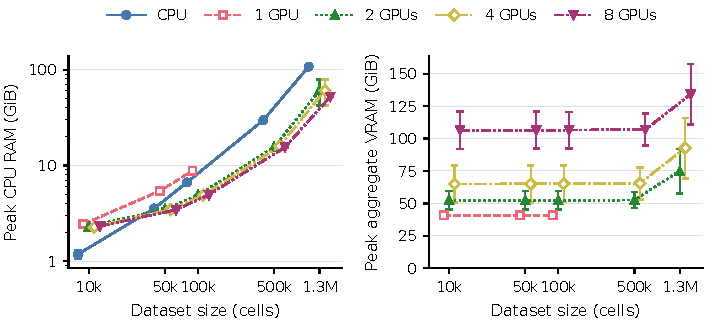
\includegraphics{figures/figS2.pdf}
\caption{\label{fig:S2}Peak memory usage across dataset sizes, mean of five repeats (first repeat included); error bars: SD. Left: CPU RAM; right: aggregate GPU VRAM summed over the allocated devices (for 2, 4 and 8 GPUs dominated by the RMM pools pre-allocated by each Dask worker). CPU RAM grows roughly linearly; GPU VRAM is approximately constant for single-GPU runs due to RMM pool pre-allocation. All repeats of a configuration ran in one process; in the multi-GPU runs VRAM grew from the first to later repeats.}
\end{figure}

\hypertarget{stress-test}{%
\subsection{Stress test}\label{stress-test}}

To locate the true capacity limit of the DGX H100 node, we ran a separate stress test with the \emph{memory-optimised pipeline} described in Methods (Section ``Stress test: maximum capacity'').

A binary search for the maximum processable cell count (Table S4) showed that the pipeline succeeded at 11.9 million cells (119 min). Above 3,436,470 cells the input was built by concatenating whole copies of the source dataset plus a random remainder, so these runs contain duplicated cells; the construction happens between data loading and QC and is not timed. ``Pass'' therefore denotes computational completion only: at 11.9M cells Leiden returned 135,710, 142,959 and 147,154 clusters at the three resolutions, against 58, 66 and 87 in a Leiden run on a 3,400,000-cell subset of the source dataset, a run not listed in Table S4. With this memory-optimised pipeline the single run at 12.0 million cells did not complete (the chunked variant described below completed at that size): after neighbour search had finished, the benchmark process exited with a timeout error while the Dask cluster was being shut down, before Leiden clustering started, and the job log records no out-of-memory error. Two runs at 13.7 million cells, one with Leiden and one with KMeans, were killed (signal 9) after HVG selection, while the full matrix was being copied to \texttt{adata.raw} and subset to the HVGs, before scaling.

The recorded peak RAM at 11.9M was 535 GiB (26\% of the 2 TB machine, 30\% of the 1.8 TB SLURM job allocation), leaving apparent headroom, while recorded peak aggregate VRAM was only 48.8 GiB out of 640 GiB (7.6\%). As described in Methods, 535 GiB is the largest between-step resident set size of the parent process alone. Two features of the 11.9M trace show what between-step sampling misses. First, RAM rises from 124 GiB at the end of data loading to 426 GiB at the start of quality control; this 302 GiB increase is the construction of the replicated 11.9M-cell dataset from the 3.4M-cell source, which runs between the two timed steps. Second, normalisation and HVG selection each register a between-step delta below 0.1 GiB, which is possible only if their working memory is allocated and released inside the call. The step-level trace therefore records the pipeline's resting footprint between operations, not the peaks against which the SLURM cgroup enforces its limit. We report an indicative budget in Table S5. At 11.9M the three Leiden calls together changed between-step host RAM by less than 1 GiB (+0.48 GiB), which, as for normalisation and HVG selection, does not exclude transient allocations within the calls; the 20 GiB rise in aggregate VRAM just before the first Leiden call occurs when the script re-initialises the RMM pool on device 0 after neighbour search, so it does not come from Leiden itself.

We also tested cuML KMeans as a GPU-native clustering alternative to Leiden (Table S4): it completed at 3.4M, 6.9M and 10.3M cells.
A sparse-scatter variant that avoided the CPU-side dense matrix was killed at 14M cells during Scanpy's HVG selection step, according to the job log.

Inspired by the chunked-preprocessing strategy of ScaleSC \cite{Hu2025}, we also implemented a third variant that performs HVG selection on per-gene running statistics accumulated over 100,000-cell batches and computes PCA via batch-wise covariance accumulation, both directly from the sparse matrix without ever materialising a dense intermediate on CPU. This variant succeeded at 12.0 million cells (862 GiB peak RAM, 10 GiB aggregate VRAM, 131.5 min) but was killed at 15.0 million cells during the CSR-to-CSC layout conversion required for HVG column slicing, according to the job log.

{\footnotesize\setlength{\tabcolsep}{2pt}
\begin{longtable}[]{@{}
  >{\raggedleft\arraybackslash}p{(\columnwidth - 10\tabcolsep) * \real{0.0986}}
  >{\raggedleft\arraybackslash}p{(\columnwidth - 10\tabcolsep) * \real{0.2113}}
  >{\raggedleft\arraybackslash}p{(\columnwidth - 10\tabcolsep) * \real{0.1972}}
  >{\raggedleft\arraybackslash}p{(\columnwidth - 10\tabcolsep) * \real{0.2113}}
  >{\raggedright\arraybackslash}p{(\columnwidth - 10\tabcolsep) * \real{0.1690}}
  >{\raggedright\arraybackslash}p{(\columnwidth - 10\tabcolsep) * \real{0.1127}}@{}}
\caption{\label{tab:S4}Stress test results: maximum cell count on a single DGX H100 node (8$\times$H100, 2 TB RAM) using the memory-optimised pipeline. Timings exclude DE testing, which was benchmarked separately (Table S6). Memory in GiB. Rows are a selection of the 16 sizes that completed (1.7M to 11.9M cells); the result files of all of them are in the repository. Above 3.4M cells the input contains replicated cells (see text).}\tabularnewline
\toprule\noalign{}
\begin{minipage}[b]{\linewidth}\raggedleft
Cells
\end{minipage} & \begin{minipage}[b]{\linewidth}\raggedleft
Runtime (min)
\end{minipage} & \begin{minipage}[b]{\linewidth}\raggedleft
CPU RAM (GiB)
\end{minipage} & \begin{minipage}[b]{\linewidth}\raggedleft
GPU VRAM (GiB)
\end{minipage} & \begin{minipage}[b]{\linewidth}\raggedright
Clustering
\end{minipage} & \begin{minipage}[b]{\linewidth}\raggedright
Status
\end{minipage} \\
\midrule\noalign{}
\endfirsthead
\toprule\noalign{}
\begin{minipage}[b]{\linewidth}\raggedleft
Cells
\end{minipage} & \begin{minipage}[b]{\linewidth}\raggedleft
Runtime (min)
\end{minipage} & \begin{minipage}[b]{\linewidth}\raggedleft
CPU RAM (GiB)
\end{minipage} & \begin{minipage}[b]{\linewidth}\raggedleft
GPU VRAM (GiB)
\end{minipage} & \begin{minipage}[b]{\linewidth}\raggedright
Clustering
\end{minipage} & \begin{minipage}[b]{\linewidth}\raggedright
Status
\end{minipage} \\
\midrule\noalign{}
\endhead
\bottomrule\noalign{}
\endlastfoot
3.4M & 18 & 155 & 49 & KMeans & Pass \\
6.9M & 38 & 308 & 49 & KMeans & Pass \\
10.3M & 91 & 465 & 49 & KMeans & Pass \\
11.5M & 114 & 517 & 49 & Leiden & Pass \\
11.9M & 119 & 535 & 49 & Leiden & \textbf{Pass (max)} \\
12.0M & n.a. & n.a. & n.a. & Leiden & Fail (Dask shutdown timeout after neighbours) \\
13.7M & n.a. & n.a. & n.a. & Leiden, KMeans & Fail (killed after HVG selection) \\
\end{longtable}
}

The three smaller rows were run with cuML KMeans instead of Leiden. Peak CPU RAM was similar for the two clustering methods at about 10M cells (465.4 GiB with KMeans at 10.31M, 460.5 GiB with Leiden at 10.2M), but runtimes were not (91.5 against 69.2 min, with QC taking 3,156 against 2,218 s; the runs were made on different days), so the runtime column combines two series and should not be read as a single curve.

{\footnotesize\setlength{\tabcolsep}{2pt}
\begin{longtable}[]{@{}
  >{\raggedright\arraybackslash}p{(\columnwidth - 2\tabcolsep) * \real{0.8710}}
  >{\raggedleft\arraybackslash}p{(\columnwidth - 2\tabcolsep) * \real{0.1290}}@{}}
\caption{\label{tab:S5}Indicative memory budget at 11.9M cells, the largest completed run (GiB). Baseline components are read from the 11.9M-cell memory trace and sum to the 535 GiB recorded there; all rows refer to 11.9M cells. The transient contributions are estimated from the operations in the pipeline code; they are not measured, because the instrumentation samples only between steps and only the parent process (Methods). The budget does not account for the full working set at any moment, and is presented to indicate which operations dominate.}\tabularnewline
\toprule\noalign{}
\begin{minipage}[b]{\linewidth}\raggedright
Memory at 11.9M cells
\end{minipage} & \begin{minipage}[b]{\linewidth}\raggedleft
GiB
\end{minipage} \\
\midrule\noalign{}
\endfirsthead
\toprule\noalign{}
\begin{minipage}[b]{\linewidth}\raggedright
Memory at 11.9M cells
\end{minipage} & \begin{minipage}[b]{\linewidth}\raggedleft
GiB
\end{minipage} \\
\midrule\noalign{}
\endhead
\bottomrule\noalign{}
\endlastfoot
\textbf{Baseline (largest between-step sample, measured at 11.9M)} & \\
~~~~Sparse raw matrix \texttt{adata.raw} (11.9M cells, replicated; RAM at the start of QC) & \textasciitilde426 \\
~~~~Dense scaled HVG matrix \texttt{adata.X} (11.9M $\times$ 2,000, float32) & 89 \\
~~~~Remainder, by difference & 20 \\
~~~~\emph{Measured subtotal (11.9M)} & \textbf{535} \\
\textbf{Contributions not represented in that subtotal} & \\
~~~~\texttt{adata.raw\ =\ adata.copy()}, a second copy of the full sparse matrix while the first is held (estimated) & +426 \\
~~~~Sparse to dense conversion before \texttt{sc.pp.scale}, one dense HVG matrix (estimated; measured net change between steps +81.7) & +89 \\
~~~~Scanpy \texttt{highly\_\allowbreak{}variable\_\allowbreak{}genes} internal temporaries & n.q. \\
~~~~Eight Dask-CUDA worker processes & n.q. \\
~~~~Leiden calls (host delta between steps at 11.9M) & \textless{} 1 \\
SLURM job allocation (\texttt{\#SBATCH\ -\/-mem=1800G}) & 1,800 \\
Physical machine memory (reported by the operating system) & 2,016 \\
\end{longtable}
}

Two contributions could not be quantified (n.q.) with the present instrumentation. In the sparse-scatter variant at 14M cells the job was killed during Scanpy's \texttt{highly\_\allowbreak{}variable\_\allowbreak{}genes}, with 629.0 GiB in use after the dataset had been built (job log); the log does not record the size of the temporaries. The resident memory of the eight Dask-CUDA worker processes is charged to the SLURM cgroup but is invisible to parent-process sampling. Either could dominate the budget above.

\hypertarget{differential-expression}{%
\subsection{Differential expression}\label{differential-expression}}

The factorial differential expression benchmark at 3.4 million cells across 41,000 genes and 81 Leiden clusters (Table S6) compares run times only; statistical properties of the tests were not assessed. To keep the table tractable we reported all wall times against a single CPU denominator, the t-test (5,598 s): a CPU Wilcoxon baseline was not run at this scale, and pseudo-bulk operates on a different sample unit (donor $\times$ cluster pseudo-samples rather than individual cells), so no strict within-method CPU-to-GPU ratio exists for it. Consequently, the speedup column should be read as ``which approach finishes fastest overall'', not as a within-method GPU acceleration factor; t-test and Wilcoxon are distinct statistical tests with different computational complexity, and any direct runtime comparison between them is descriptive, not inferential.

{\footnotesize\setlength{\tabcolsep}{2pt}
\begin{longtable}[]{@{}llrrr@{}}
\caption{\label{tab:S6}Differential expression benchmark at 3.4M cells $\times$ 41k genes $\times$ 81 Leiden clusters. Speedup is relative to CPU t-test (5,598 s).}\tabularnewline
\toprule\noalign{}
Method & Backend & GPUs & Time (s) & Speedup \\
\midrule\noalign{}
\endfirsthead
\toprule\noalign{}
Method & Backend & GPUs & Time (s) & Speedup \\
\midrule\noalign{}
\endhead
\bottomrule\noalign{}
\endlastfoot
t-test & CPU & 0 & 5,598 & 1.0$\times$ \\
Pseudo-bulk (Wilcoxon) & CPU (aggregated) & 0 & 127 & 43.9$\times$ \\
Wilcoxon (scatter) & GPU & 8 & 826 & 6.8$\times$ \\
Wilcoxon (chunk-stream) & GPU & 1 & 831 & 6.7$\times$ \\
t-test (scatter) & GPU & 8 & 1,655 & 3.4$\times$ \\
t-test (chunk-stream) & GPU & 1 & 1,649 & 3.4$\times$ \\
\end{longtable}
}

Pseudo-bulk aggregation was the fastest strategy: aggregating log-normalised expression by donor and cluster reduced 3.4 million cells to 2,431 pseudo-samples (about 30 per cluster), and the analysis completed in 127 s (2.1 min), 43.9 times sooner than the cell-level CPU t-test (5,598 s, 93 min). Among cell-level tests on GPU, the Wilcoxon implementation (826 s) finished sooner than the t-test (1,655 s), and multi-GPU scatter (826 s for Wilcoxon) was essentially equivalent to single-GPU chunk-and-stream (831 s).

\hypertarget{spatial-end-to-end-speedup-and-co-occurrence}{%
\subsection{Spatial end-to-end speedup and co-occurrence}\label{spatial-end-to-end-speedup-and-co-occurrence}}

Against the DGX CPU reference, end-to-end GPU speedups were 1.4$\times$ on Visium v1 (2,695 spots), 6.9$\times$ on Visium HD 8~\textmu{}m (393,543 bins; co-occurrence excluded, see below) and 10.4$\times$ on the random 400k-bin subsample of Visium HD 2~\textmu{}m (389,492 bins after QC) (Table 2 of the chapter, Fig. S3).
With the 128-thread workstation CPU as reference they were 1.6$\times$, 6.1$\times$ and 9.4$\times$: the choice of CPU changed the speedup by 10-14\%, in different directions per platform.
Visium HD 8~\textmu{}m and the 2~\textmu{}m subsample have similar numbers of bins but ran different steps (co-occurrence and neighbourhood enrichment were skipped at 2~\textmu{}m, see below), so the order of the speedups does not show an effect of resolution.

\begin{figure}
\centering
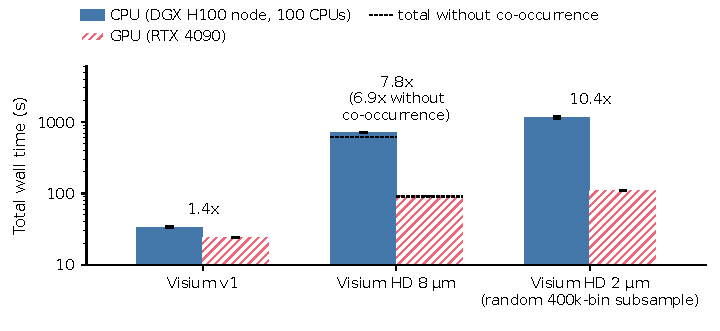
\includegraphics{figures/figS3.pdf}
\caption{\label{fig:S3}Total pipeline wall time on three Visium platforms: CPU reference (one DGX H100 node, 100 CPUs) and GPU (one RTX 4090), mean of five repeats, each in a fresh process; error bars: SD. Labels give the speedup (ratio of means). At Visium HD 8~\textmu{}m the bars include co-occurrence, whose GPU result with rapids-singlecell 0.14.1 was incorrect (see text); the dashed lines mark the totals without it (6.9$\times$). Visium HD 2~\textmu{}m was randomly subsampled to 400,000 bins (389,492 after QC) to fit in the 24 GiB of the RTX 4090.}
\end{figure}

At Visium HD 8~\textmu{}m, with the same 4 cell groups as the CPU, the GPU co-occurrence computed with rapids-singlecell 0.14.1 was incorrect: it matched the CPU result within an absolute tolerance of 0.001 in only 8 of 49 distance intervals, because the number of bin pairs within the larger distance thresholds exceeds the range of its 32-bit integer counters.
The GPU co-occurrence of the original March runs had the same defect.
With rapids-singlecell 0.15.1 the GPU result matched the CPU in 49 of 49 intervals (maximum absolute difference 0.00022) at unchanged runtime (0.15.1/0.14.1 time ratio 0.98, 95\% CI 0.95-1.00).
In this separate check, co-occurrence with 0.15.1 took 4.41 s against 103 s on the DGX CPU (23.4$\times$, 95\% CI 23.3-23.6); because the check ran outside the pipeline and the pipeline result was incorrect, co-occurrence is excluded from the Visium HD speedups.
Squidpy counts co-occurring cluster pairs with a Numba-parallel loop over all pairs of bins for each distance interval (O(n\^{}2) per interval); rapids-singlecell performs the same counting on the GPU.
On the DGX CPU, co-occurrence took 14.4\% of the pipeline time at Visium HD 8~\textmu{}m.

\hypertarget{spatial-per-step-speedup}{%
\subsection{Spatial per-step speedup}\label{spatial-per-step-speedup}}

On Visium HD 8~\textmu{}m the GPU accelerated UMAP 197$\times$, Geary's C 122$\times$, PCA (with scaling) 37.0$\times$, normalisation 30.4$\times$ and Moran's I 20.8$\times$; expression neighbours and Leiden clustering were accelerated 13.5$\times$ and 12.9$\times$, and data loading, QC and HVG selection ran at 0.99$\times$, 0.89$\times$ and 1.8$\times$ (Table S7, Fig. 3 of the chapter).
As in the scRNA-seq pipeline, CPU expression neighbour search ran pynndescent on one Numba thread (Methods), so its speedup is relative to a single-threaded search.

{\footnotesize\setlength{\tabcolsep}{2pt}
\begin{longtable}[]{@{}
  >{\raggedright\arraybackslash}p{(\columnwidth - 6\tabcolsep) * \real{0.3721}}
  >{\raggedleft\arraybackslash}p{(\columnwidth - 6\tabcolsep) * \real{0.2093}}
  >{\raggedleft\arraybackslash}p{(\columnwidth - 6\tabcolsep) * \real{0.2093}}
  >{\raggedleft\arraybackslash}p{(\columnwidth - 6\tabcolsep) * \real{0.2093}}@{}}
\caption{\label{tab:S7}Per-step wall time and GPU speedup on Visium HD 8~\textmu{}m (393,543 bins): mean~$\pm$~SD of five repeats, each in a fresh process; CPU reference: one DGX H100 node (100 CPUs); speedup: ratio of means with 95\% bootstrap interval. Spatial neighbours and neighbourhood enrichment have no GPU implementation in rapids-singlecell 0.14.1: the GPU pipeline calls Squidpy on the CPU, so the GPU column for these rows is CPU time on the workstation. PCA includes scaling. CPU expression neighbour search ran on one Numba thread (Methods). Co-occurrence: the GPU result with rapids-singlecell 0.14.1 was incorrect (see text), so no GPU time or speedup is reported (n.r.); with 0.15.1, in a separate check, it took 4.41 s (23.4$\times$). The total includes co-occurrence.}\tabularnewline
\toprule\noalign{}
\begin{minipage}[b]{\linewidth}\raggedright
Step
\end{minipage} & \begin{minipage}[b]{\linewidth}\raggedleft
CPU (s)
\end{minipage} & \begin{minipage}[b]{\linewidth}\raggedleft
GPU (s)
\end{minipage} & \begin{minipage}[b]{\linewidth}\raggedleft
Speedup
\end{minipage} \\
\midrule\noalign{}
\endfirsthead
\toprule\noalign{}
\begin{minipage}[b]{\linewidth}\raggedright
Step
\end{minipage} & \begin{minipage}[b]{\linewidth}\raggedleft
CPU (s)
\end{minipage} & \begin{minipage}[b]{\linewidth}\raggedleft
GPU (s)
\end{minipage} & \begin{minipage}[b]{\linewidth}\raggedleft
Speedup
\end{minipage} \\
\midrule\noalign{}
\endhead
\bottomrule\noalign{}
\endlastfoot
Data loading & 3.87~$\pm$~0.15 & 3.93~$\pm$~0.08 & 0.99$\times$ (0.96-1.02) \\
QC and filtering & 2.72~$\pm$~0.09 & 3.07~$\pm$~0.04 & 0.89$\times$ (0.86-0.91) \\
Normalisation & 2.62~$\pm$~0.14 & 0.0861~$\pm$~0.0030 & 30.4$\times$ (29.1-32.1) \\
HVG selection & 1.03~$\pm$~0.06 & 0.579~$\pm$~0.059 & 1.8$\times$ (1.6-1.9) \\
PCA & 33.7~$\pm$~0.1 & 0.909~$\pm$~0.028 & 37.0$\times$ (36.1-37.9) \\
Expression neighbours & 58.1~$\pm$~0.2 & 4.29~$\pm$~0.11 & 13.5$\times$ (13.2-13.7) \\
Leiden clustering & 21.2~$\pm$~0.2 & 1.65~$\pm$~0.02 & 12.9$\times$ (12.7-13.1) \\
UMAP & 269~$\pm$~5 & 1.366~$\pm$~0.007 & 197$\times$ (194-200) \\
Spatial neighbours (CPU in both) & 45.2~$\pm$~0.3 & 56.3~$\pm$~0.9 & 0.80$\times$ (0.79-0.81) \\
Moran's I & 82.6~$\pm$~1.4 & 3.98~$\pm$~0.32 & 20.8$\times$ (19.4-21.9) \\
Geary's C & 82.1~$\pm$~2.0 & 0.671~$\pm$~0.003 & 122$\times$ (120-125) \\
Co-occurrence & 103.2~$\pm$~0.3 & n.r. & n.r. \\
Neighbourhood enrichment (CPU in both) & 13.5~$\pm$~0.2 & 12.8~$\pm$~0.4 & 1.1$\times$ (1.0-1.1) \\
Total & 719~$\pm$~3 & 92.2~$\pm$~0.7 & 7.80$\times$ (7.75-7.85) \\
\end{longtable}
}

On the Visium HD 2~\textmu{}m subsample, CPU Leiden returned 3,027 groups, so co-occurrence and neighbourhood enrichment were skipped (more than 500 groups, Methods) and the totals contain fewer steps than at Visium HD 8~\textmu{}m.
UMAP, the largest CPU cost (72.0\% of the CPU time), ran 89.4$\times$ faster on the GPU; the GPU pipeline time (110 s) was dominated by spatial neighbours (50.4\%) and data loading (27.8\%).

On Visium v1 (2,695 spots) the end-to-end speedup was 1.4$\times$: ligand-receptor analysis, run in Squidpy on the CPU in both pipelines, took 38.2\% of the GPU pipeline time, and QC (0.18$\times$), Leiden (0.27$\times$), Moran's I (0.51$\times$) and PCA (0.67$\times$) were slower on the GPU than on the CPU.

Three steps ran in Squidpy on the CPU inside the GPU pipeline: spatial neighbours (Delaunay triangulation via scipy.spatial), neighbourhood enrichment and ligand-receptor analysis (Visium v1 only).
On the two Visium HD platforms spatial neighbours took 45.2 s and 45.0 s on the DGX CPU and 56.3 s and 55.4 s in the GPU pipeline on the workstation CPU, 61.1\% (HD 8~\textmu{}m) and 50.4\% (HD 2~\textmu{}m subsample) of the GPU pipeline time.

\hypertarget{spatial-concordance}{%
\subsection{Spatial concordance}\label{spatial-concordance}}

Spatial autocorrelation statistics agreed closely between CPU and GPU on all three platforms (Table S8, Fig. 4 of the chapter).

Moran's I and Geary's C Spearman correlations between CPU and GPU were at least 0.9995 in all cases.
The top-50 spatially variable genes by Moran's I formed the same set on CPU and GPU on all three platforms (Jaccard = 1.000); for the top 100 and top 200 the Jaccard index was 1.000 on Visium v1 and 0.980 on both Visium HD platforms.
At FDR \textless{} 0.05, the Jaccard index of the SVG sets was 1.000 (Visium v1), 0.999 (HD 8~\textmu{}m) and 0.982 (HD 2~\textmu{}m subsample).

{\footnotesize\setlength{\tabcolsep}{2pt}
\begin{longtable}[]{@{}
  >{\raggedright\arraybackslash}p{(\columnwidth - 6\tabcolsep) * \real{0.2857}}
  >{\raggedleft\arraybackslash}p{(\columnwidth - 6\tabcolsep) * \real{0.2245}}
  >{\raggedleft\arraybackslash}p{(\columnwidth - 6\tabcolsep) * \real{0.2449}}
  >{\raggedleft\arraybackslash}p{(\columnwidth - 6\tabcolsep) * \real{0.2449}}@{}}
\caption{\label{tab:S8}Spatial concordance between the CPU reference (DGX node) and GPU pipelines, CPU repeat k against GPU repeat k (k = 1-5): a single value when it is the same in the five pairs, otherwise the range. SVG Jaccard reports the overlap of spatially variable genes ranked by Moran's I. Co-occurrence and neighbourhood enrichment were skipped on the HD 2~\textmu{}m subsample (more than 500 groups); at Visium HD 8~\textmu{}m the GPU co-occurrence is the incorrect result of rapids-singlecell 0.14.1 (see text). N clusters: groups returned by each pipeline's own Leiden run in each repeat. With the workstation CPU as reference, CPU Leiden returned 16, 7 and 2,559 groups and the ARI was 0.856, 0.972-0.975 and 0.084.}\tabularnewline
\toprule\noalign{}
\begin{minipage}[b]{\linewidth}\raggedright
Metric
\end{minipage} & \begin{minipage}[b]{\linewidth}\raggedleft
Visium v1
\end{minipage} & \begin{minipage}[b]{\linewidth}\raggedleft
HD 8~\textmu{}m
\end{minipage} & \begin{minipage}[b]{\linewidth}\raggedleft
Visium HD 2~\textmu{}m (random 400k-bin subsample)
\end{minipage} \\
\midrule\noalign{}
\endfirsthead
\toprule\noalign{}
\begin{minipage}[b]{\linewidth}\raggedright
Metric
\end{minipage} & \begin{minipage}[b]{\linewidth}\raggedleft
Visium v1
\end{minipage} & \begin{minipage}[b]{\linewidth}\raggedleft
HD 8~\textmu{}m
\end{minipage} & \begin{minipage}[b]{\linewidth}\raggedleft
Visium HD 2~\textmu{}m (random 400k-bin subsample)
\end{minipage} \\
\midrule\noalign{}
\endhead
\bottomrule\noalign{}
\endlastfoot
Moran's I Spearman $\rho$ & 1.0000 & 0.9999 & 1.0000 \\
Geary's C Spearman $\rho$ & 1.0000 & 0.9995 & 0.9999 \\
SVG Jaccard (top 50) & 1.000 & 1.000 & 1.000 \\
SVG Jaccard (top 100) & 1.000 & 0.980 & 0.980 \\
SVG Jaccard (top 200) & 1.000 & 0.980 & 0.980 \\
SVG Jaccard (FDR \textless{} 0.05) & 1.000 & 0.999 & 0.982 \\
Cluster ARI & 0.856 & 0.971-0.974 & 0.071 \\
Cluster NMI & 0.892 & 0.936-0.942 & 0.636 \\
N clusters (CPU / GPU) & 16 / 15 & 4 / 3-4 & 3,027 / 538 \\
Co-occurrence Spearman $\rho$ & 1.0000 & 0.1118 (0.14.1) & n.r. \\
Neighbourhood enrichment Spearman $\rho$ & 0.9977-0.9982 & 1.0000 & n.r. \\
\end{longtable}
}

Expression-based Leiden clustering agreed on Visium v1 (ARI 0.856, NMI 0.892) and Visium HD 8~\textmu{}m (ARI 0.971-0.974, NMI 0.936-0.942 over the five repeat pairs), where GPU Leiden returned 3 groups in four repeats and 4 in one, against 4 for the DGX CPU (7 for the workstation CPU).
On the Visium HD 2~\textmu{}m subsample the partitions diverged (ARI 0.071, NMI 0.636): CPU Leiden returned 3,027 clusters on the DGX reference and GPU Leiden 538, in each of the five repeats.
The number of CPU clusters depended on the CPU machine (2,559 on the 128-thread workstation).
This 5.63-fold difference in cluster granularity coincides with the use of two Leiden implementations with different settings (igraph with 2 iterations on the CPU, cuGraph with up to 100 iterations on the GPU); we did not test which of the two factors, or the subsampling, causes it.
The 2~\textmu{}m subsample retains 389,492 of 6.3 million bins; we did not test whether its sparsity contributes to the fragmented partition.

\hypertarget{spatial-memory}{%
\subsection{Spatial memory}\label{spatial-memory}}

GPU memory readings (NVML, device-wide) reflect the RMM memory pool: 12.59 GiB was reserved before data loading in every GPU run, and the peak reading was 12.74 GiB on Visium v1, 22.74 GiB on Visium HD 8~\textmu{}m and 22.73 GiB on the HD 2~\textmu{}m subsample (95\% of the 24.0 GiB of the RTX 4090); the 2~\textmu{}m data had to be subsampled to fit (Methods).
Peak CPU RAM ranged from 0.97 GiB (Visium v1) to 7.95 GiB (HD 2~\textmu{}m subsample) on the DGX CPU reference, and reached 11.30 GiB in the GPU pipeline (Visium HD 8~\textmu{}m).
Whether the full-resolution Visium HD 2~\textmu{}m dataset (6.3 million bins) fits in GPU memory was not tested; the CPU pipeline densifies the HVG matrix, which at this size would need about 50 GB (47 GiB) in float32.

\hypertarget{supplementary-discussion}{%
\section{Supplementary Discussion}\label{supplementary-discussion}}

GPU speedup was operation-specific. Normalisation (173-329$\times$), an element-wise operation limited by memory bandwidth rather than by arithmetic, had the largest speedup at every size, and neighbour graph construction (44-88$\times$) benefited strongly from the GPU. The CPU neighbour search, however, ran pynndescent with a single numba thread (Scanpy's default \texttt{n\_\allowbreak{}jobs\ =\ 1}; Methods); on a separate server, 100 threads made it 1.16, 1.91 and 2.48 times faster at 10,000, 50,000 and 100,000 cells, so against a multi-threaded CPU search the neighbour speedup would shrink to about 76$\times$, 32$\times$ and 18$\times$, and at 100,000 cells (95\% bootstrap interval 8.6-33.1$\times$) it would fall below that of PCA (36.5$\times$). In contrast, data loading was slower on the GPU at every size tested (0.76-0.85$\times$), and Leiden at 10,000 cells was slower on the GPU only at the first resolution (0.36$\times$, mean of five repeats), an effect of the first cuGraph call in the first repeat (1.70 s against a mean of 0.13 s in repeats 2-5); at resolutions 1.0 and 1.5 the GPU was faster (1.36$\times$ and 1.60$\times$). For data loading, CUDA context initialisation and RMM pool allocation took place before the timer (Methods), so the timed GPU step comprised reading the h5ad file through CPU RAM and transferring the matrix to the device; its excess over the CPU (+0.10, +0.55 and +1.38 s at 10,000, 50,000 and 100,000 cells) grew with dataset size, which is consistent with reading and conversion costs rather than with a fixed overhead. In practice, the GPU advantage grew with dataset size, but even at the smallest size tested (10,000 cells) the GPU pipeline was 12.0-fold faster end to end, partly because CPU differential expression took 54.9\% of the CPU time; we did not observe a size at which GPU overhead outweighed its benefit. Dicks et al.~note that below about 50,000 cells kernel-launch and host-device transfer overheads can make CPU execution comparable or faster \cite{Dicks2026}; their benchmark workflow excluded differential expression.

In the spatial benchmark, the GPU advantage was concentrated in a few steps rather than spread across spatial statistics as a whole. At Visium HD 8~\textmu{}m, GPU co-occurrence in rapids-singlecell 0.14.1 was incorrect: on the same 4 cell groups as the CPU it matched the CPU result at only 8 of 49 distances, because its 32-bit pair counters overflow at this number of bins. With rapids-singlecell 0.15.1 it matched at 49 of 49 distances in the same time (time ratio 0.98, 95\% CI 0.95-1.00), so we excluded co-occurrence from the Visium HD speedups; in a separate check the corrected version was 23.4$\times$ faster than the DGX CPU. Spatial autocorrelation statistics were accelerated 20.8-21.0$\times$ (Moran's I) and 122.4-128.9$\times$ (Geary's C) on Visium HD (9.3-13.1$\times$ and 55.1-75.6$\times$ against the workstation CPU), with near-perfect numerical concordance (Spearman $\rho$ \textgreater= 0.9995); the top-50 spatially variable genes formed the same set on CPU and GPU, and each statistic took 0.7-4.0 s on the GPU instead of 82-86 s on the CPU reference. On the GPU, Moran's I remained slower than Geary's C (about 4 s against less than 1 s), and on Visium v1 it was not accelerated (0.51$\times$). In rapids-singlecell 0.14.1, spatial neighbour computation and neighbourhood enrichment have no GPU implementation and ran on the CPU inside the GPU pipeline (0.80$\times$ and 1.1$\times$ at Visium HD 8~\textmu{}m); ligand-receptor analysis, run on Visium v1 only, has a GPU implementation in rapids-singlecell 0.14.1 that our pipeline did not use (Squidpy on the CPU in both pipelines, 0.96$\times$).

Our study contains several limitations that should be considered when generalising these findings. All scRNA-seq experiments used mouse brain cells from CELLxGENE Census: a random sample for the scaling benchmark and the full 3,436,470-cell selection for the stress test, replicated by concatenation beyond that size, and a 3.4M-cell subset of it (202 donors) for differential expression; performance profiles may differ for other tissues and for datasets with different sparsity patterns or gene counts. Concordance analysis was performed at 10,000 cells; larger datasets may exhibit different adjusted Rand index distributions or reveal additional numerical differences. The CPU baseline was a SLURM allocation of 100 logical CPUs on a node with 224, and we did not measure how Scanpy runtimes scale with the number of threads. In the hybrid runs at 1.3M cells, Scanpy QC took 188.2 s with 32 allocated CPUs and 186.6 s with 100, which suggests that some steps are largely single-threaded; the speedups are therefore relative to this allocation, not per core. The stress test employing the memory-optimised pipeline is mathematically equivalent to but not implementation-identical to the standard rapids-singlecell workflow, introducing potential differences in how the optimization generalises to other analyses. The GPU part of the spatial benchmark ran on an RTX 4090 workstation, while its CPU reference ran on a DGX node; multi-GPU spatial analysis and the full Visium HD 2~\textmu{}m resolution (6.3 million bins) were not benchmarked. The drivers of the cluster nodes (535.247.01 and 535.183.01) cap the CUDA runtime at 12.2, and the GPU components of the spatial stack did not run with them (Supplementary Methods, ``Hardware and software environment''). Scaling analysis was confined to a single DGX H100 node (1-8 GPUs); we did not benchmark multi-node configurations (e.g., 16 GPUs across two nodes interconnected by InfiniBand), and since our multi-GPU configuration did not distribute any step (Results), it gives no indication of how a distributed pipeline would behave across nodes. A further limitation concerns the multi-GPU configuration itself: at 500k and 1.3M cells we ran only the Dask-CUDA hybrid, in which, as implemented, preprocessing ran in Scanpy on the host CPU; rapids-singlecell 0.14.1 provides Dask-based routes for QC, normalisation, log1p, scaling and PCA that we did not use. The share of the timed total spent in CPU preprocessing (data loading, QC, normalisation and HVG selection) in the 8-GPU hybrid runs at 1.3M cells (78.0\%, mean of five repeats) is thus a property of our configuration, which ran preprocessing in Scanpy on the CPU, rather than an intrinsic limit of GPU acceleration. The memory peaks of the stress test are lower bounds and the attribution in Table S5 is indicative (Supplementary Methods, ``Stress test: maximum capacity''). Finally, we did not benchmark integration methods (Harmony \cite{Korsunsky2019}, scVI \cite{Lopez2018}) or multi-sample spatial experimental designs, which represent important directions for ongoing work.


\typeout{REFSTART \thepage}
\bibliographystyle{splncs04}
\bibliography{cibb2026_references}
\typeout{DOCEND \thepage}
\end{document}
